\documentclass[tikz,border=2pt]{standalone}
\usepackage{amsmath,amssymb}
\usepackage{pgfplots}
\pgfplotsset{compat=1.18}

\begin{document}
% Independent X ~ Pois(2) and Y ~ Pois(3): the product of the MGFs is the MGF of Pois(5), so
% X + Y ~ Pois(5). The three pmfs are shown side by side.
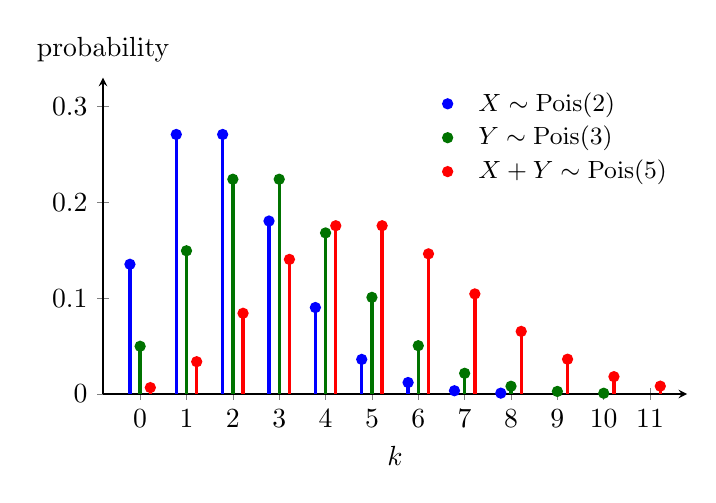
\begin{tikzpicture}
	\begin{axis}[
		axis lines=left, xmin=-0.8, xmax=11.8, ymin=0, ymax=0.33,
		xtick={0,1,...,11}, ytick={0,0.1,0.2,0.3},
		xlabel={$k$}, ylabel={probability}, ylabel style={rotate=-90, anchor=south, at={(axis description cs:0,1.02)}},
		width=9cm, height=5.6cm, clip=false,
		legend style={draw=none, fill=none, font=\small, at={(0.99,0.99)}, anchor=north east}, legend cell align=left
		]
		\addplot[ycomb, blue, very thick, mark=*, mark size=1.4pt] coordinates {(-0.22,0.1353) (0.78,0.2707) (1.78,0.2707) (2.78,0.1804) (3.78,0.0902) (4.78,0.0361) (5.78,0.0120) (6.78,0.0034) (7.78,0.0009)};
		\addlegendentry{$X\sim\operatorname{Pois}(2)$}
		\addplot[ycomb, green!45!black, very thick, mark=*, mark size=1.4pt] coordinates {(0,0.0498) (1,0.1494) (2,0.2240) (3,0.2240) (4,0.1680) (5,0.1008) (6,0.0504) (7,0.0216) (8,0.0081) (9,0.0027) (10,0.0008)};
		\addlegendentry{$Y\sim\operatorname{Pois}(3)$}
		\addplot[ycomb, red, very thick, mark=*, mark size=1.4pt] coordinates {(0.22,0.0067) (1.22,0.0337) (2.22,0.0842) (3.22,0.1404) (4.22,0.1755) (5.22,0.1755) (6.22,0.1462) (7.22,0.1044) (8.22,0.0653) (9.22,0.0363) (10.22,0.0181) (11.22,0.0082)};
		\addlegendentry{$X+Y\sim\operatorname{Pois}(5)$}
	\end{axis}
	
\end{tikzpicture}
\end{document}
